\section{Motivations and basic definitions}

In order to obtain some information --~as detailed as possible --~on a \emph{natural system}, such as in geophysics, or regarding the important subcategory of \emph{living systems} which constitute the objects of study in biology and medicine, the most straightforward strategy consists in obtaining \emph{measurements} on the system at hand. Note that we deliberately use the term measurement, related but not reduced to \emph{experiments}, to signify that it is not in general possible to design specific experiments allowing to determine all kinds of physical properties of the system --~as is done for instance for industrial systems. By contrast, natural systems induce drastic limitations in measurements, in that they generally must be ``taken as they are'', namely, observed in their current operating conditions, whether this is due to the practical impossibility of apprehending them comprehensively (e.g.~in geophysics), or to the undesirable character of any strong perturbation of the system (invasiveness in living systems).

Specializing now our discussion on living systems, abundant measurements are frequently at hand, in the form of clinical images and signals of various origins. Despite the diversity and rich information contents of these data, they are also inevitably limited in many respects. Beside considerations on sampling and noise, this holds in particular as regards:
\begin{itemize}
	\item their extent: for example only 2D measurements, or boundary information, may be available for a 3D system, or only part of the whole domain;
	\item their type: some quantities are never measured, such as internal stresses in a living tissue, or various physical constitutive parameters (stiffness, contractility, etc.).
\end{itemize}

Nevertheless, we may want to consider \emph{physical models} to describe and predict the behavior of these systems. Clearly, these models may be seen as providing some complementary information on the system. However, their predictivity requires the careful adjustment of many parameters --~in particular regarding the detailed geometry (anatomy), physical properties, boundary conditions and initial conditions needed in the model --~most of which being out of reach of the available measurements.

The purpose of \emph{data assimilation} is then to combine the information available from these two sources --~measurements on the one hand, and models and the other hand --~by seeking an adequate compromise between:
\begin{itemize}
	\item the discrepancy computed between simulations of the model and the corresponding measurements;
	\item the \emph{a priori} confidence in the model, since errors are also present in the measurements.
\end{itemize}
The desired output of this procedure is an estimation of the unknown quantities of interest, namely,
\begin{itemize}
	\item state variables (the ``trajectories'' of the system), and in particular their initial values at a given reference time;
	\item physical parameters which must be prescribed in the model equations.
\end{itemize}
In terms of clinical applications, the expected benefits are to assist and improve both \emph{diagnosis} and \emph{prognosis}:
\begin{itemize}
	\item diagnosis, by providing more complete information on the patient (spatially-distributed quantities, and various otherwise unreachable indicators), and with improved accuracy;
	\item prognosis, since once data assimilation has been performed the model can be more confidently used to predict natural or artificial evolutions of the system, for example to simulate the effect of various possible therapeutic strategies.
\end{itemize}

We will now introduce some basic notation necessary to discuss the fundamental principles of data assimilation. First of all, we consider physical models in the form of dynamical systems governed by equations of the type
\begin{equation}\label{eq:modelNotation}
	\dot{x} = \mathcal{M}(x,p,t).
\end{equation}
In this equation, $x$ denotes the so-called \emph{state variable}, namely, the physical quantity which the model aims at describing in its time-wise evolution --~hence, the time derivative in the left-hand side --~and also frequently spatial variations for distributed quantities. In this generic notation, the whole model is essentially summarized in the so-called \emph{dynamical operator} $\mathcal{M}$, which applies on the state variable itself, and may depend on time $t$ as well as on a set of physical parameters denoted by $p$. This operator may arise from various types of physical formulations, e.g.~in solid and fluid mechanics or electrophysiology. Mathematically speaking, it may take the form of partial differential equations (PDEs) or ordinary differential equations (ODEs, namely, only differentiated with respect to the time variable), or algebraic systems, in particular.

Clearly, in such model formulations we need to prescribe --~hence to estimate when unknown via the data assimilation procedure --~the initial condition $\mathcal{M}(0)$ and the parameter vector $p$. Typically, in the models considered the state variable may contain a large number of scalar coefficients --~typically $10^3$ to $10^7$ degrees of freedom in a continuum mechanics model --~whereas the size of the parameter vector is generally much more limited, and in practice we seldom have to estimate more than a few hundreds of parameter values. Once the initial condition and the parameter vector associated with \eqref{eq:modelNotation} are estimated, the model can be simulated in time, using appropriate numerical techniques.

Another important notation concerns the measurements, typically represented by an equation of the type
\begin{equation}\label{eq:measNotation}
	y = \mathcal{H}(x,t) + e^o,
\end{equation}
where $y$ denotes the actual data, $\mathcal{H}$ is the so-called \emph{observation operator}, and $e^o$ accounts for the error inherent to the measurement process, often called the \emph{noise}. Note that the quantity $y$ will frequently correspond to pre-processed --~not raw --~data, for example images processed with segmentation or optical flow techniques in order to extract some position, displacement or velocity information. We further emphasize that this equation also represents a model --~in this case of the measurements --~where modeling ingredients are embedded both in the expression of $\mathcal{H}$ and the characterization of $e^o$, which may be of probabilistic or deterministic nature.


\section{Fundamental principles}

We are now in a position to introduce some fundamental principles for data assimilation procedures. First of all, there are two main categories of methods: variational and sequential methods.

\subsection{Variational procedures}

In variational procedures, we consider a criterion to be minimized in order to achieve the above-mentioned compromise between simulation-measurements discrepancy and model confidence, see e.g.~\cite{Bensoussan71,Chavent10} and references therein. A typical criterion would read
\begin{equation}\label{eq:varCriterion}
	\mathcal{J}_T(\varstate_\state,\varstate_{\param}) = \int_0^T \|\observ-\obsOp(\state)\|_{\obsNoiseNorm}^2 \, dt + \|\varstate_\state\|_{(\initNoiseCov)^{-1}}^2 + \|\varstate_{\param}\|_{(\paramNoiseCov)^{-1}}^2,
\end{equation}
where $\|.\|_{\obsNoiseNorm}$, $\|.\|_{(\initNoiseCov)^{-1}}$ and $\|.\|_{(\paramNoiseCov)^{-1}}$ denote suitable norms for each quantity concerned, and associated with the matrices appearing as subscripts. In this criterion, $\state$ is constrained to satisfy the model equation \eqref{eq:modelNotation} starting from the initial condition $\state(0)=\state_0+\initNoise_\state$ and with parameter values given by $\param=\param_0+\initNoise_\param$. In order to perform this minimization, a classical strategy consists in computing the gradient of the criterion, which requires the simulation of the so-called \emph{adjoint model}. The adjoint model equation is an evolution system closely related to --~and inferred from, indeed --~the direct model equation \eqref{eq:modelNotation}, viz.
\begin{equation}\label{eq:adjointPb}
	\begin{cases}
	\dot{\adjoint}_\state + \frac{\partial \modelOp}{\partial \state}^\intercal \adjoint_\state = -\frac{\partial \obsOp}{\partial \state}^\intercal\obsNoiseNorm(\observ-\obsOp(\state)) \\
	\adjoint_\state(T) = 0 \\
	\dot{\adjoint}_{\param} + \frac{\partial \modelOp}{\partial \param}^\intercal\adjoint_\state= 0 \\
	\adjoint_{\param}(T) = 0
	\end{cases}
\end{equation}
These equations must be simulated backwards in time from the final time $T$ to the initial time in order to obtain the gradient value criterion expressed as
\[
	\begin{cases}
		\diff_{\varstate_\state}\mathcal{J} \cdot \delta \varstate_\state = {\varstate_\state}^\intercal (\initNoiseCov)^{-1} \delta \varstate_\state - \adjoint_\state(0)^\intercal \delta \varstate_\state\\
		\diff_{\varstate_{\param}}\mathcal{J} \cdot \delta \param = {\varstate_\param}^\intercal (\paramNoiseCov)^{-1} \delta \varstate_\param - \adjoint_{\param}(0)^\intercal \delta \varstate_\param,
	\end{cases}
\]
Hence, each gradient computation requires the forward simulation of the direct model and the backward simulation of the adjoint, and this must be repeated until convergence of the minimization algorithm. Figure \ref{fig:variat} illustrates this iterative procedure, and the fact that observability can be improved by considering a longer time window, hence, also more measurements. This type of variational procedure is also referred to as ``4DVar'' in the data assimilation community, while ``3DVar'' is used to refer to minimization estimation performed for static models, or for dynamic models at a given time (namely, without time integral).

\begin{figure}[htbp]
\begin{center}
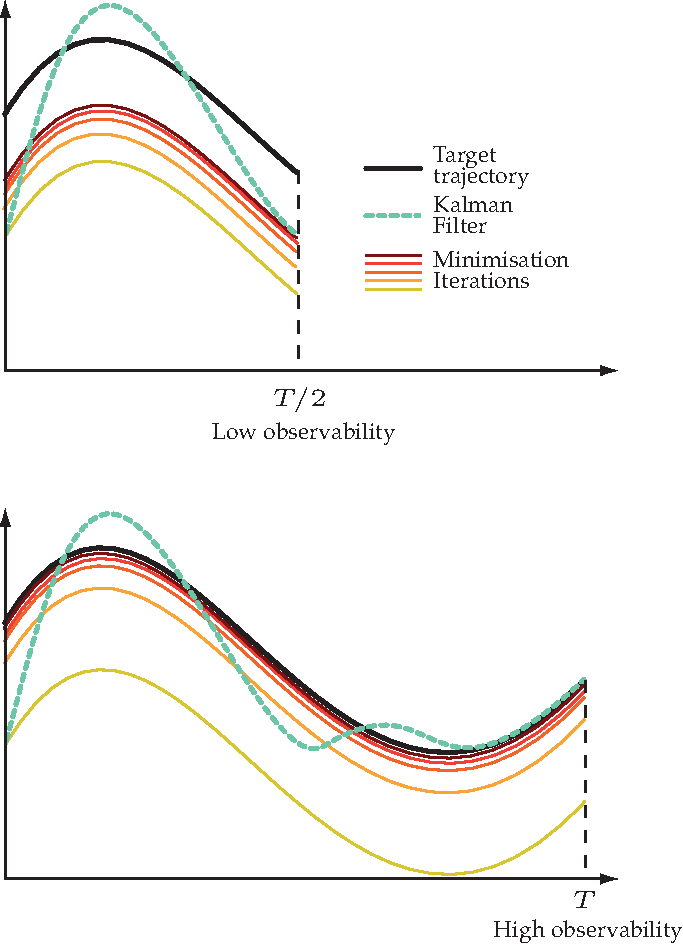
\includegraphics[width=.5\textwidth]{figure/seqVSvaria.pdf}
\caption{Schematic of minimization iterations and Kalman filter tracking on a sliding time window (as seen via one single output)}
\label{fig:variat}
\end{center}
\end{figure}

Concerning the time discretization, it is classical to formulate an optimal discrete time minimization criterion and find its corresponding adjoint rather than discretizing directly \eqref{eq:adjointPb}. Hence, we consider a criterion of the form
\begin{equation}\label{eq:varCriterionTimeDisc}
	J_N(\varstate_\state,\varstate_{\param}) = \sum_{k=0}^N \|\observDof_k-\obsOpDof(\stateDof_k)\|_{\obsNoiseNormDof_k}^2 \,  + \|\varstateDof_\state\|_{(\initNoiseCovDof)^{-1}}^2 + \|\varstateDof_{\param}\|_{(\paramNoiseCovDof)^{-1}}^2,
\end{equation}
with for example $\obsNoiseNormDof_k = \Delta t \obsNoiseNormDof$.

\subsection{Sequential procedures}

By contrast, sequential procedures --~also often referred to as \emph{filtering} --~proceed by simulating equations closely resembling the direct model equations, with an additional correction term taking into account the discrepancy between the simulation and the actual measurements, namely $y-\mathcal{H}(x)$, quantity called the \emph{innovation}. For example when only the initial condition is unknown the filtering equation would be of the type
\begin{equation}\label{eq:filterNotation}
	\dot{\state^a} = \modelOp(\state^a,t) + K(\observ-\obsOp(\state^a)),
\end{equation}
where the operator $K$ --~frequently linear --~is called the \emph{filter}. The filtering equation simulation is then started from the candidate initial condition $X_0$, and the aim of the correction is to bring the simulated trajectory close to the target system, see Fig.~\ref{fig:variat}.

This type of strategy was made extremely popular by the Kalman theory, which formulated an optimal setting for deriving the filter operator, initially when the operators $A$ and $H$ are both linear. In this case, the Kalman equations read
\begin{equation}\label{eq:Kalman}
	\begin{cases}
		\dot{\state^a} = \modelOp\state^a + \Cov\obsOp^\intercal \obsNoiseNorm (\observ-\obsOp\state^a)\\
		\dot{\Cov} - \Cov\modelOp^\intercal - \modelOp\Cov + \Cov\obsOp^\intercal \obsNoiseNorm \obsOp\Cov = 0\\
		\Cov(0)=\initNoiseCov\\
		\state^a(0) = \stateAug_\diamond
	\end{cases}
\end{equation}
where $W$ and $P_0$ denote the  so-called covariance matrices of the measurement noise and initial condition uncertainty, respectively. We can see that the filter expression is based on the computation of the time-dependent covariance matrix $P$ which satisfies a Riccatti equation. In fact, in the linear case the variational and Kalman procedures can be shown to be exactly equivalent, and the minimizing direct and adjoint states ($X_\text{inf}$ and $p_\text{inf}$, respectively) are related to the Kalman filter by the identity \cite{Bensoussan71}
\[
	\stateAug_\infty = \state^a + \Cov \adjoint_\infty.
\]
This is also illustrated in Figure \ref{fig:variat} where we show that the Kalman estimation coincides with the minimizing solution at the end of the time window considered.

When nonlinearities are to be considered, various extensions are available, and in particular the Extended Kalman Filtering (EKF) approach, in which the linearized forms of the operators are used in the filter equation. However, in such a case the approach is no longer equivalent to the variational setting. Nevertheless, some alternative filter equations can be derived from the variational formulation, but the filter computation then requires solving a Hamilton-Jacobi-Bellman equation in a space which has the dimension of the state variable \cite{Moireau08}, which is in general not practical.

Note that, in practice, the Kalman (or EKF) approach itself is also quite limited as regards the size of the system which can be handled, since the covariance matrix $\Cov$ has the size of the state variable, and is a dense matrix, unlike the dynamical operators. In order to circumvent this limitation some alternative approaches must be considered.

Concerning time discretization, it is classical to formulate the optimal filter directly from the optimal time-discrete minimization criteria rather than discretizing directly \eqref{eq:Kalman}. Hence, after some quite tedious computations, we can formulate a prediction-correction scheme
\begin{subequations}\label{eq:KalmanDiscrete}
	\begin{enumerate}
	\item Prediction:
   \begin{align}
   	\begin{cases}
   		\hat{\stateDof}_{h+1}^f &= \modelOp_{h}(\stateDof_h^a) \\
   		\CovDof_{h+1}^f &= \frac{\partial \modelOpDof_{h}}{\partial \stateDof} \CovDof_{h}^a \frac{\partial \modelOpDof_{h}}{\partial \stateDof}^\intercal
   	\end{cases}
   \end{align}
	\item Correction:
   \begin{align}\label{eq:KalmanCorrection}
   	\begin{cases}
   		\CovDof_{h+1}^a &= \left(\frac{\partial \obsOpDof_{h+1}}{\partial \stateDof} ^\intercal\obsNoiseCovDof_{h+1}^{-1} \frac{\partial \obsOpDof_{h+1}}{\partial \stateDof} + (\CovDof_{h+1}^f)^{-1}\right)^{-1} \\
		\gainOpDof_{h+1} &= \CovDof_{h+1}^a \frac{\partial \obsOpDof_{h+1}}{\partial \stateDof}^\intercal \obsNoiseCovDof_{h+1}^{-1} \\
		\hat{\stateDof}_{h+1}^a  &= \hat{\stateDof}_{h+1}^f + \gainOpDof_{h+1}(\observDof_{h+1}- \obsOpDof_{h+1}(\hat{\stateDof}_{h+1}^f))
   	\end{cases}
   \end{align}
\end{enumerate}
\end{subequations}


For the sake of simplicity, we have introduced the Kalman filter in a deterministic context, but the probabilistic counterpart exists. In a linear framework the expressions are exactly the same, albeit with the additional interpretation
\begin{equation}\label{eq:proba}
	\begin{cases}
			\text{a priori mean: } \hat{\stateDof}_{h+1}^f = \E(\stateDof_{h+1}|\observDof_0,\ldots,\observDof_h),	\\
			\text{a priori covariance: }  \CovDof_{h+1}^f = \E\bigl((\stateDof_{h+1}-\hat{\stateDof}_{h+1}^f)(\stateDof_{h+1}-\hat{\stateDof}_{h+1}^f)^\intercal\bigr), \\
			\text{a posteriori mean: } \hat{\stateDof}_{h+1}^a = \E\bigl(\stateDof_{h+1}|\observDof_0,\ldots,\observDof_{h+1}\bigr), \\
			\text{a posteriori covariance: } \CovDof_{h+1}^a = \E((\stateDof_{h+1}-\hat{\stateDof}_{h+1}^a)(\stateDof_{h+1}-\hat{\stateDof}_{h+1}^a)^\intercal),
	\end{cases}
\end{equation}

This results extend to the non-linear context with the EKF \eqref{eq:KalmanDiscrete} but the identities \eqref{eq:proba} are then only approximate. To improve the quality of this approximation, the Unscented Kalman Filter has then been introduced \cite{Julier00}, based on the idea of substituting means and covariances by empirical quantities computed from sample points:
\begin{equation}\label{eq:probaEmpirical}
	\begin{cases}
			\hat{\stateDof}_{h+1}^f = \sum_{i=1}^d \alpha_i\stateDof_{h+1}^{[i]-},	\\
			\CovDof_{h+1}^f = \sum_{i=1}^d \alpha_i(\stateDof_{h+1}^{[i]-}-\hat{\stateDof}_{h+1}^f)(\stateDof_{h+1}^{[i]-}-\hat{\stateDof}_{h+1}^f)^\intercal, \\
			\hat{\stateDof}_{h+1}^a = \sum_{i=1}^d \alpha_i\stateDof_{h+1}^{[i]+}, \\
			\CovDof_{h+1}^a = \sum_{i=1}^d \alpha_i(\stateDof_{h+1}^{[i]+}-\hat{\stateDof}_{h+1}^a)(\stateDof_{h+1}^{[i]+}-\hat{\stateDof}_{h+1}^a)^\intercal,
	\end{cases}
\end{equation}
with $\sum_{i=1}^d \alpha_i = 1$.

In practice, the correction particles are sampled around the mean $\hat{\stateDof}_{h}^a$ with a covariance $\CovDof_{h}^a$ and the prediction samples then verify
\begin{subequations}\label{eq:UKFDiscrete}
\begin{equation}
	\stateDof_{h+1}^{[i]-} = \modelOpDof(\stateDof_{h}^{[i]+}).
\end{equation}
Then, by computing
\begin{equation}
	\observDof_{h+1}^{[i]-} = \obsOpDof(\stateDof_{h+1}^{[i]-}),\quad  \observDof_{h+1}^{-} = \sum_{i=1}^d \alpha_i \observDof_{h+1}^{[i]}
\end{equation}
The gain is defined by
\begin{equation}
\begin{cases}
		\gainOpDof_{h+1} = (\CovDof_{h+1}^{\stateDof,\observDof}) \cdot (\CovDof_{h+1}^{\observDof,\observDof})^{-1} \\
		\CovDof_{h+1}^{\stateDof,\observDof} = \sum_{i=1}^d \alpha_i(\stateDof_{h+1}^{[i]-}-\hat{\stateDof}_{h+1}^f)(\observDof_{h+1}^{[i]-}-\observDof_{h+1}^{-})^\intercal\\
		\CovDof_{h+1}^{\observDof,\observDof} = \sum_{i=1}^d \alpha_i(\observDof_{h+1}^{[i]-}-\observDof_{h+1}^{-})(\observDof_{h+1}^{[i]-}-\observDof_{h+1}^{-})^\intercal + W_{h+1}
\end{cases}
\end{equation}
so that we keep having
\begin{equation}
\begin{cases}
	\hat{\stateDof}_{h+1}^a  = \hat{\stateDof}_{h+1}^f + \gainOpDof_{h+1}(\observDof_{h+1}- \observDof_{h+1}^{-}) \\
	\CovDof_{h+1}^a = \CovDof_{h+1}^f - \CovDof_{h+1}^{\stateDof,\observDof}  (\CovDof_{h+1}^{\observDof,\observDof})^{-1} 	(\CovDof_{h+1}^{\stateDof,\observDof})^\intercal
\end{cases}
\end{equation}
\end{subequations}
and proceed recursively with new correction particles $\stateDof_{h+1}^{[i]+}$.


The Ensemble Kalman Filter, introduced in \cite{EVENSEN:1994tl}, follows the same principles of approximating the covariances by sampled particles with, most of the time, an increased number of particles with respect to the UKF filter, and various ways of sampling the particles around the mean value. Finally Monte Carlo strategies exploit  a very large number of particles to give a better approximation of the non-linear optimal filter but the practical details of these methods are beyond the scope of this review focused on large dimensional systems coming from the discretization of PDEs.


\subsection{Reduced-order sequential strategies}\label{sec:RO}

\paragraph{Reduced-Order Extended Kalman Filtering (ROEKF)}

In order to deal with the limitations of sequential strategies due to the system size, a classical strategy consists in assuming a specific reduced-order form for the covariance operators. For example, making the ansatz
\begin{equation}\label{eq:red-order-princ}
	\forall t,\quad \Cov(t) = L(t) U(t)^{-1} L(t)^\intercal
\end{equation}
with $U$ an invertible matrix of small size $r$ and $L$ an extension operator, we can show that within linear assumptions the solution of the Riccatti equation in \eqref{eq:Kalman} reduces to
\begin{equation}\label{eq:reducedDynamics}
	\dot{L} = \modelOp L \text{ and }
	\dot{U} = L^\intercal \obsOp^\intercal \obsNoiseNorm \obsOp L.
\end{equation}
which is actually computable in practice.

In a non-linear framework, we can then approximate the covariance dynamics by extending \eqref{eq:reducedDynamics} as
\begin{equation}\label{eq:nl-reducedDynamics}
	\dot{L} = \frac{\partial \modelOp}{\partial \stateAug} L \text{ and }
	\dot{U} = L^\intercal \frac{\partial \obsOp}{\partial \stateAug}^\intercal \obsNoiseNorm \frac{\partial \obsOp}{\partial \stateAug} L.
\end{equation}
These strategies have relevant applications in the case of parameter identification \emph{per se}. It is common, indeed, to assume more space regularity for the parameters than for the state initial condition. Hence, after discretization the parameters can be represented by a small number of degrees of freedom. Assuming that we can limit $U(0)$ to the parametric space, the extension operator can then be decomposed into two components $L = \left( \begin{smallmatrix} \LX \\ \Ltheta \end{smallmatrix} \right)$ with $\Ltheta = \1$ and
\begin{equation}\label{eq:sensitivity}
	\dot{L}_\state = \frac{\partial \modelOp}{\partial \state} \LX + \frac{\partial \modelOp}{\partial \param}.
\end{equation}
We recognize in this expression the dynamics of the sensitivity operator $\frac{\partial \state}{\partial \param}$, which provides a nice interpretation for this strategy of uncertainty covariance reduction. Furthermore, in the linear framework we can prove that this sequential estimator corresponds to the optimal filter associated with the criterion
\begin{equation}\label{eq:paramCriterion}
	\mathcal{J}(\varstate_{\param}) = \int_0^T \|\observ-\obsOp(\state)\|_{\obsNoiseNorm}^2 \, dt +  \|\varstate_{\param}\|_{(\paramNoiseCov)^{-1}}^2,
\end{equation}
where $\state$ follows the trajectory associated with $\varstate_{\param}$ and fixed initial condition, which is commonly used in variational identification procedures. All this justifies naming this strategy \emph{Reduced-Order Extended Kalman Filter} (ROEKF), but it is also known as \emph{Singular Evolutive Extended Kalman Filter} following the work of \cite{Pham:1998p44}.

This concept can be applied directly on time and space discretized versions of the equations, which leads to a \emph{discrete time Reduced-Order Extended Kalman Filter}.
\begin{subequations}\label{eq:ROKalmanDiscrete}
	\begin{enumerate}
	\item Prediction:
   \begin{align}
   	\begin{cases}
   		\hat{\stateDof}_{h+1}^f &= \modelOpDof_{h} (\stateDof_{h}^a) \\
   		L_{h+1} &= \frac{\partial \modelOpDof_{h}}{\partial \stateDof}  L_h
   	\end{cases}
   \end{align}
	\item Correction:
   \begin{align}
   	\begin{cases}
   		U_{h+1} &= U_{h} + L_{h+1}^\intercal \frac{\partial \obsOpDof_{h+1}}{\partial \stateDof}^\intercal \obsNoiseCovDof^{-1}_{h+1} \frac{\partial \obsOpDof_{h+1}}{\partial \stateDof} L_{h+1} \\
		\gainOpDof_{h+1} &= \CovDof_{h+1}^a \frac{\partial \obsOpDof_{h+1}}{\partial \stateDof}^\intercal\obsNoiseCovDof_{h+1}^{-1} \\
		\hat{\stateDof}_{h+1}^a  &= \hat{\stateDof}_{h+1}^f + \gainOpDof_{h+1}(\observDof_{h+1}- \obsOpDof_{h+1} \hat{\stateDof}_{h+1}^f)
   	\end{cases}
   \end{align}
\end{enumerate}
\end{subequations}

\paragraph{Reduced-Order Unscented Kalman Filtering (ROUKF)}

Alternatively, this strategy can be coupled with the UKF approach by showing that particles can be generated only in the space of small dimension and the computation made in the UKF filter \eqref{eq:UKFDiscrete} can be compatible with the time discretized counterpart of \eqref{eq:red-order-princ}. This was proven in \cite{PM-DC-10,moireau-chapelle-11err} which also provided a very general version of the \emph{Reduced Order Unscented Kalman Filter} (ROUKF). In particular this algorithm is close to the \emph{Singular Evolutive Interpolated Kalman Filter} \cite{pham01stochastic,hoteit-pham-blum-02} for a choice of particles $d = r+1$ and reads as follows.
\paragraph{Algorithm~--} Given an adequate sampling rule, we store the corresponding weights in the diagonal matrix $\mathbf{D}_\alpha$ and precompute so-called unitary sigma-points (i.e.~with zero mean and unit covariance) denoted by $(\vec{I}^{[i]})_{1\leq i \leq r+1}$; we then perform at each time step
\begin{subequations}
	\begin{enumerate}
		\item Sampling:
	\begin{align}
		\begin{cases}
			C_h &= \sqrt{(U_h)^{-1}} \\[0.1cm]
			\hat{\stateDof}^{[i]+}_{h} &= \hat{\stateDof}_{h}^a + L_h \cdot C_h^\intercal \cdot \vec{I}^{[i]},\quad 1\leq i \leq r+1 \\[0.1cm]
		\end{cases}
	\end{align}
	\item Prediction:
   \begin{align}
   	\begin{cases}
   		\hat{\stateDof}^{[i]-}_{h+1} &= \modelOpDof_{h}(\hat{\stateDof}^{[i]+}_{h}),\quad 1\leq i \leq r+1 \\[0.1cm]
   	   	\hat{\stateDof}^f_{h+1} &= \sum_{i=1}^{r+1} \alpha_i \hat{\stateDof}_{h+1}^{[i]-}\\[0.1cm]
   	\end{cases}
   \end{align}
	\item Correction:
   \begin{align}
   	\begin{cases}
   		L_{h+1} &= [\hat{\stateDof}^{[*]-}_{h+1}]\mathbf{D}_\alpha [\vec{I}^{[*]}]^\intercal \\[0.1cm]
   		\observDof_{h+1}^{[i]-} &= \obsOpDof_{h+1}(\hat{\stateDof}^{[i]-}_{h+1}) \\[0.1cm]
		\observDof_{h+1}^f &= \sum_{i=1}^{r+1} \alpha_i \observDof_{h+1}^{[i]-} \\[0.1cm]
   		\mathbf{\Gamma}_{h+1} &=  [\observDof^{[*]-}_{h+1}]\mathbf{D}_\alpha [\vec{I}^{[*]}]^\intercal \\[0.1cm]
   		U^{n+1} &=  \mathbf{1} + \mathbf{\Gamma}_{h+1}^\intercal  \obsNoiseCovDof_{h+1}^{-1} \mathbf{\Gamma}_{h+1} \\[0.1cm]
   		\hat{\stateDof}_{h+1}^a &= \hat{\stateDof}_{h+1}^f - L_{h+1} U^{n+1}  \mathbf{\Gamma}_{h+1}^\intercal \obsNoiseCovDof_{h+1}^{-1}  (\observDof_{h+1} - \observDof_{h+1}^f)
   	\end{cases}
   \end{align}
\end{enumerate}
\end{subequations}
where we denote by $[\vec{I}^{[*]}]$ the matrix concatenating the $(\vec{I}^{[i]})$ vectors side by side, and similarly for other vectors.


\subsection{Luenberger observers}

The so-called \emph{observer theory}, initiated by Luenberger \cite{Luenberger63}, is based on the simple realization that, defining the estimation error
\[
	\tilde{\state} = \state - \state^a,
\]
we obtain in the linear case, when subtracting the direct model and filtered equations, the dynamics
\begin{equation}
	\dot{\tilde{\state}} = (\modelOp-\gainFilter\obsOp) \tilde{\state} - \gainFilter\chi.
\end{equation}
This type of dynamical equation is well-known is control theory: it is similar to the closed-loop controlled equation of a system of natural dynamics governed by $\modelOp$, and submitted to a feedback control defined by the operator $\gainFilter$ applied on the quantity observed through $\obsOp$. Hence, obtaining an accurate estimation of the state variable is exactly equivalent to driving the estimation error $\tilde{\state}$ to zero --~namely, stabilizing this error --~using the feedback control $\gainFilter$.

This approach opened new avenues for formulating novel filtering approaches, because for actual dynamical systems control and stabilization motivations have frequently already led to the formulation of effective feedback controls, used in a large variety of industrial systems. Hence, these approaches can be quite directly adapted to obtain adequate filters which --~unlike the Kalman filter --~are tractable in practice for large systems. Moreover, these filters are often deeply rooted in the physics of the system considered, hence the computational building blocks needed are likely to be already available in the system simulation software. However, in the Luenberger approach we lose the Kalman optimality, which of course only holds in quite restricted (linear) cases.

For examples of such approaches applicable to biomechanics we refer to \cite{PM-DC-PLT-09}. We also point out that the Luenberger observer approach is also sometimes referred to as ``nudging'' in the data assimilation community \cite{Auroux:2008p2884}.


\subsection{Joint state-parameter estimation with Luenberger observers}

As apparent in the above discussion, Luenberger observers were originally designed for state estimation. When parameters are to be jointly estimated, it is quite classical in the filtering context to complement the state equation \eqref{eq:modelNotation} with the artificial parameter dynamics
\begin{equation}
	\dot{p} = 0.
\end{equation}
Then the whole estimation objective is to estimate the initial condition of the so-called \emph{augmented state} $(X,p)$. Of course, when a Kalman approach is out of reach for the state variable alone, it holds \emph{a fortiori} for the augmented state. On the other hand, devising a Luenberger observer for the augmented state is difficult, because part of the dynamics is non-physical, hence feedback controls are not readily available for the joint system.

Nevertheless, an effective approach for joint state-parameter estimation was proposed in \cite{PM-DC-PLT-08}, based on a Luenberger observer applied on the state equation alone. In essence, this first stage state estimation reduces the uncertainty to the parameter space, which allows to consider a Kalman-like approach (or EKF-like in nonlinear cases) for handling the remaining parameter uncertainty. This algorithm can be summarized as
\begin{equation}\label{eq:jointEst}
	\begin{cases}
			\dot{\state^a} = \modelOp(\state^a,\hat{\param}) + \gainFilter_\state(\observ-\obsOp\state^a) + \LX\dot{\hat{\param}}\\
			\dot{\hat{\param}} = U^{-1} {\LX}^\intercal \obsOp^\intercal \obsNoiseNorm (\observ-\obsOp\state^a) \\
			\dot{L}_\state = \bigl( \frac{\partial \modelOp}{\partial \state} - \gainFilter_\state\obsOp \bigr) \LX + \frac{\partial \modelOp}{\partial \param}\\
			\dot{U} = {\LX}^\intercal \obsOp^\intercal \obsNoiseNorm \obsOp \LX \\
			\state^a(0) = \state_0\\
			\hat{\param}(0) = \param_0 \\
			\LX(0) = 0 \\
			U(0) = U_0
	\end{cases}
\end{equation}
where $K_X$ denotes the state filter (Luenberger observer), $\LX$ represents the sensitivity of the state variable with respect to the parameters, and $U$ the inverse of the parameter estimation error covariance. This methodology is strongly related to so-called \emph{reduced filtering} approaches, see e.g.~\cite{Pham:1998p44}, since essentially only the part of the dynamics concerning parameters is handled using optimal filtering.

This joint estimation approach was later extended in \cite{PM-DC-10} towards strategies inspired from so-called unscented filtering methods --~also related to Ensemble Kalman filtering and particle filtering --~allowing to avoid the computation of differentiated operators required in \eqref{eq:jointEst}.
